% Simple CMOS (N-MOSFET & P-MOSFET) H bridge.
% Author: Uli Koehler (https://techoverflow.net)
% Based on http://texample.net/tikz/examples/power-electronics-converter-inverter/
%   by Ali Mehrizi-Sani
%
% NOTE: Requires recent CircuiTikZ version in order to use [T]elmech and fetbodydiode!
% TeXLive 2015 is too old, please use at least TeXLive 2016!

\documentclass[tikz, border=1mm]{standalone}
\usepackage{siunitx}
\usepackage[european,cuteinductors]{circuitikz}

\usetikzlibrary{decorations.markings}
\usetikzlibrary{calc}
\ctikzset{bipoles/thickness=1}
\tikzstyle{every node}=[font=\small]
\tikzstyle{every path}=[line width=0.8pt,line cap=round,line join=round]

\begin{document}
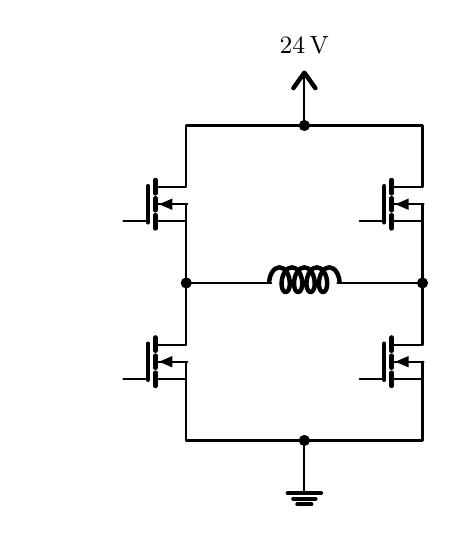
\begin{tikzpicture}
    % Define named coordinates
    \draw (0,0)
    ++(2,4) coordinate (NE)
    ++(0,-4) coordinate (SE)
    (NE)++(1.5,0) coordinate (VCC)
    (SE)++(1.5,0) coordinate (GND)
    (2,2) coordinate (InductorL)
    ++(3,0) coordinate (InductorR);

    % VCC & GND connection
    \draw (VCC) to[short,*-] ++(0,0.25) node[vcc]{\SI{24}{\volt}}
    (GND) to[short,*-]++(0,-0.25) node[ground]{}

    % MOSFETs for west leg
    (NE)++(0,-1) node [nigfete,scale=0.8,name=fet1] {}
    ++(0,-2) node [nigfete,scale=0.8,name=fet4] {};
    % Connections for west leg
    \draw  (NE) -| (fet1.D)
    (fet1.S) to (fet4.D)
    (fet4.S) |- (SE);

    % MOSFETs for east leg
    \draw (NE)++(3,0)
    ++(0,-1) node [nigfete,scale=0.8,name=fet3] {}
    ++(0,-2) node [nigfete,scale=0.8,name=fet2] {};
    % Connections for east leg
    \draw(NE) -| (fet3.D)
    (fet3.S) -- (fet2.D)
    (fet2.S) |- (SE);

    % Inductor (between the legs)
    \draw (InductorL) to[L,*-*] (InductorR);
\end{tikzpicture}
\newpage
% Same as above, current highlighted
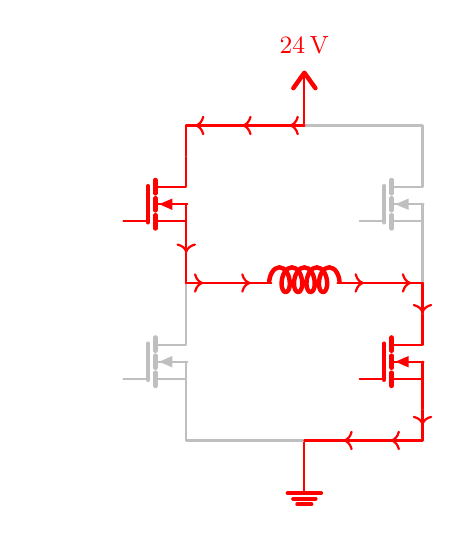
\begin{tikzpicture}
    % Define named coordinates
    \draw (0,0)
    ++(2,4) coordinate (NE)
    ++(0,-4) coordinate (SE)
    (NE)++(1.5,0) coordinate (VCC)
    (SE)++(1.5,0) coordinate (GND)
    (2,2) coordinate (InductorL)
    ++(3,0) coordinate (InductorR);

    % VCC & GND connection
    \draw[red] (VCC) to[draw=red,short,color=red] ++(0,0.25) node[color=red,vcc]{\SI{24}{\volt}}
    (GND) to[short,color=red]++(0,-0.25) node[color=red,ground]{}

    % MOSFETs for west leg
    (NE)++(0,-1) node [color=red,nigfete,scale=0.8,name=fet1] {}
    ++(0,-2) node [color=lightgray,nigfete,scale=0.8,name=fet4] {};
    % Connections for west leg
    \draw [lightgray] (NE) -| (fet1.D)
    (fet1.S) to (fet4.D)
    (fet4.S) |- (SE);

    % MOSFETs for east leg
    \draw (NE)++(3,0)
    ++(0,-1) node [color=lightgray,nigfete,scale=0.8,name=fet3] {}
    ++(0,-2) node [color=red,nigfete,scale=0.8,name=fet2] {};
    % Connections for east leg
    \draw[lightgray](NE) -| (fet3.D)
    (fet3.S) to (fet2.D)
    (fet2.S) |- (SE);

    % Inductor (between the legs)

    % Draw current direction(over "normal" connections).
    \begin{scope}[very thick,decoration={
            markings,
            mark=between positions 0.1 and 1.2 step 6mm with {\arrow{>}}}
        ] 
        % West section
        \draw[red,postaction={decorate}] (VCC) -| (fet1.D);
        \draw[red,postaction={decorate}] (fet2.S) |- (GND);
        % Inductor 
        \draw[red,postaction={decorate}] (2,2) to[L,color=red] ++(3,0);
    \end{scope}
    % Shorter sections with different arrow parameters
    \begin{scope}[very thick,decoration={
            markings,
            mark=at position 0 with {\arrow{>}}}
        ] 
        % West section
        \draw[red,postaction={decorate}] (fet1.S) -- (InductorL);
    \end{scope}
    \begin{scope}[very thick,decoration={
            markings,
            mark=at position 1 with {\arrow{>}}}
        ] 
        % West section
        \draw[red,postaction={decorate}] (InductorR) -- (fet2.D);
    \end{scope}

\end{tikzpicture}
\end{document}